\begin{table}[htbp]
    \small
    \centering
    \begin{tabular}{cl}
        \toprule
        Sources & ROI according to the Harvard-Oxford atlas \\
        \midrule
        \cspSourcesPerROI
        \bottomrule
    \end{tabular}
    \caption{Number of sources, which were considered task-relevant based on the source reconstruction of CSP patterns, for ROIs according to the Harvard-Oxford atlas. ROIs that were used in the analysis are highlighted in bold. ROIs that are not listed in the table did not contain any task-relevant sources.}
    \label{tab:csp_sources_per_roi}
\end{table}

\begin{table}[htbp]
    \small
    \centering
    \resizebox{\linewidth}{!}{\multiverseRestSummary}
    \caption{Summary of the observed effects for the research questions in the joint multiverse analysis. Significant effects are highlighted in bold, and stars indicate that the effects remain significant after Bonferroni correction for multiple ($m = \numComparisons$) comparisons. WH and AH stand for within- and across-hemisphere values of PS metrics, respectively.}
    \label{tab:multiverse_effects_summary}
\end{table}

\begin{figure}[htbp]
    \centering
    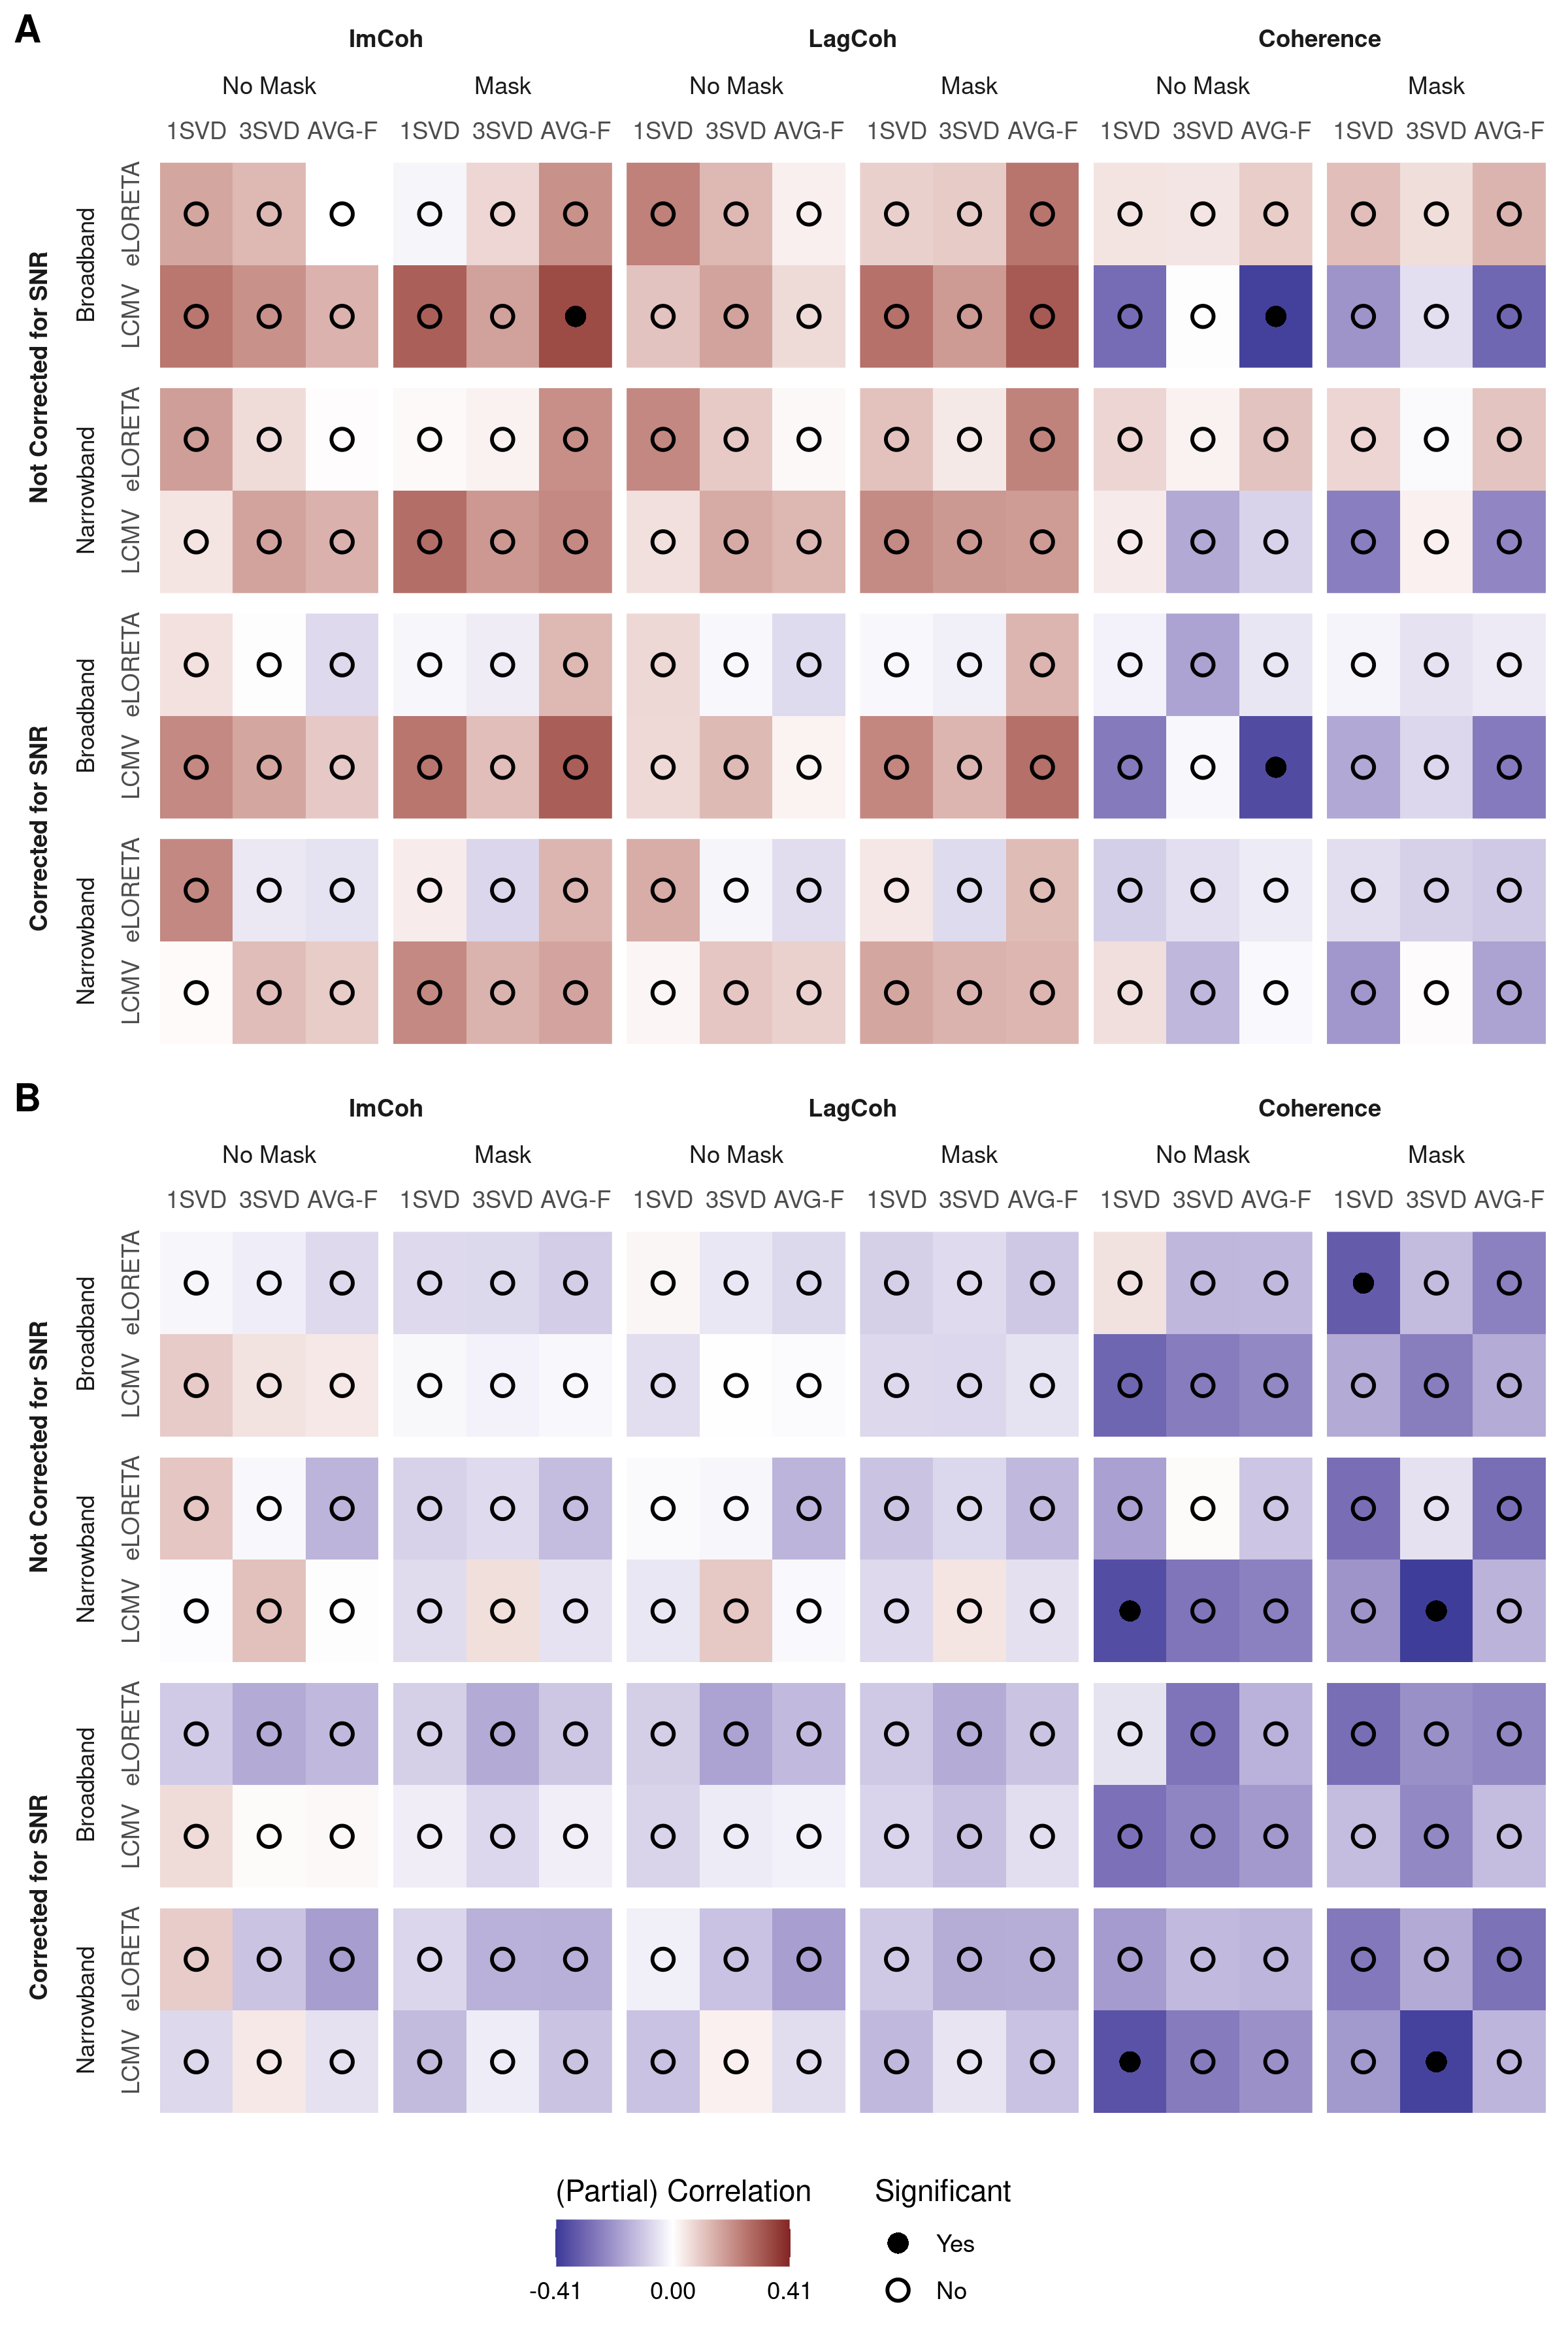
\includegraphics[width=0.9\textwidth]{fig6supp1-multiverse-connectivity-performance-between-subject.png}
    \caption{Between-subject effects of phase synchronization on performance as assessed with correlation (Not Corrected for SNR) and partial correlation (Corrected for SNR). Panels (A) and (B) correspond to within- and across-hemisphere phase synchronization, respectively. Bonferroni correction for multiple ($m = \numComparisons$) comparisons was applied.}
    \label{fig:multiverse_connectivity_performance_between}
\end{figure}

\begin{figure}[htbp]
    \centering
    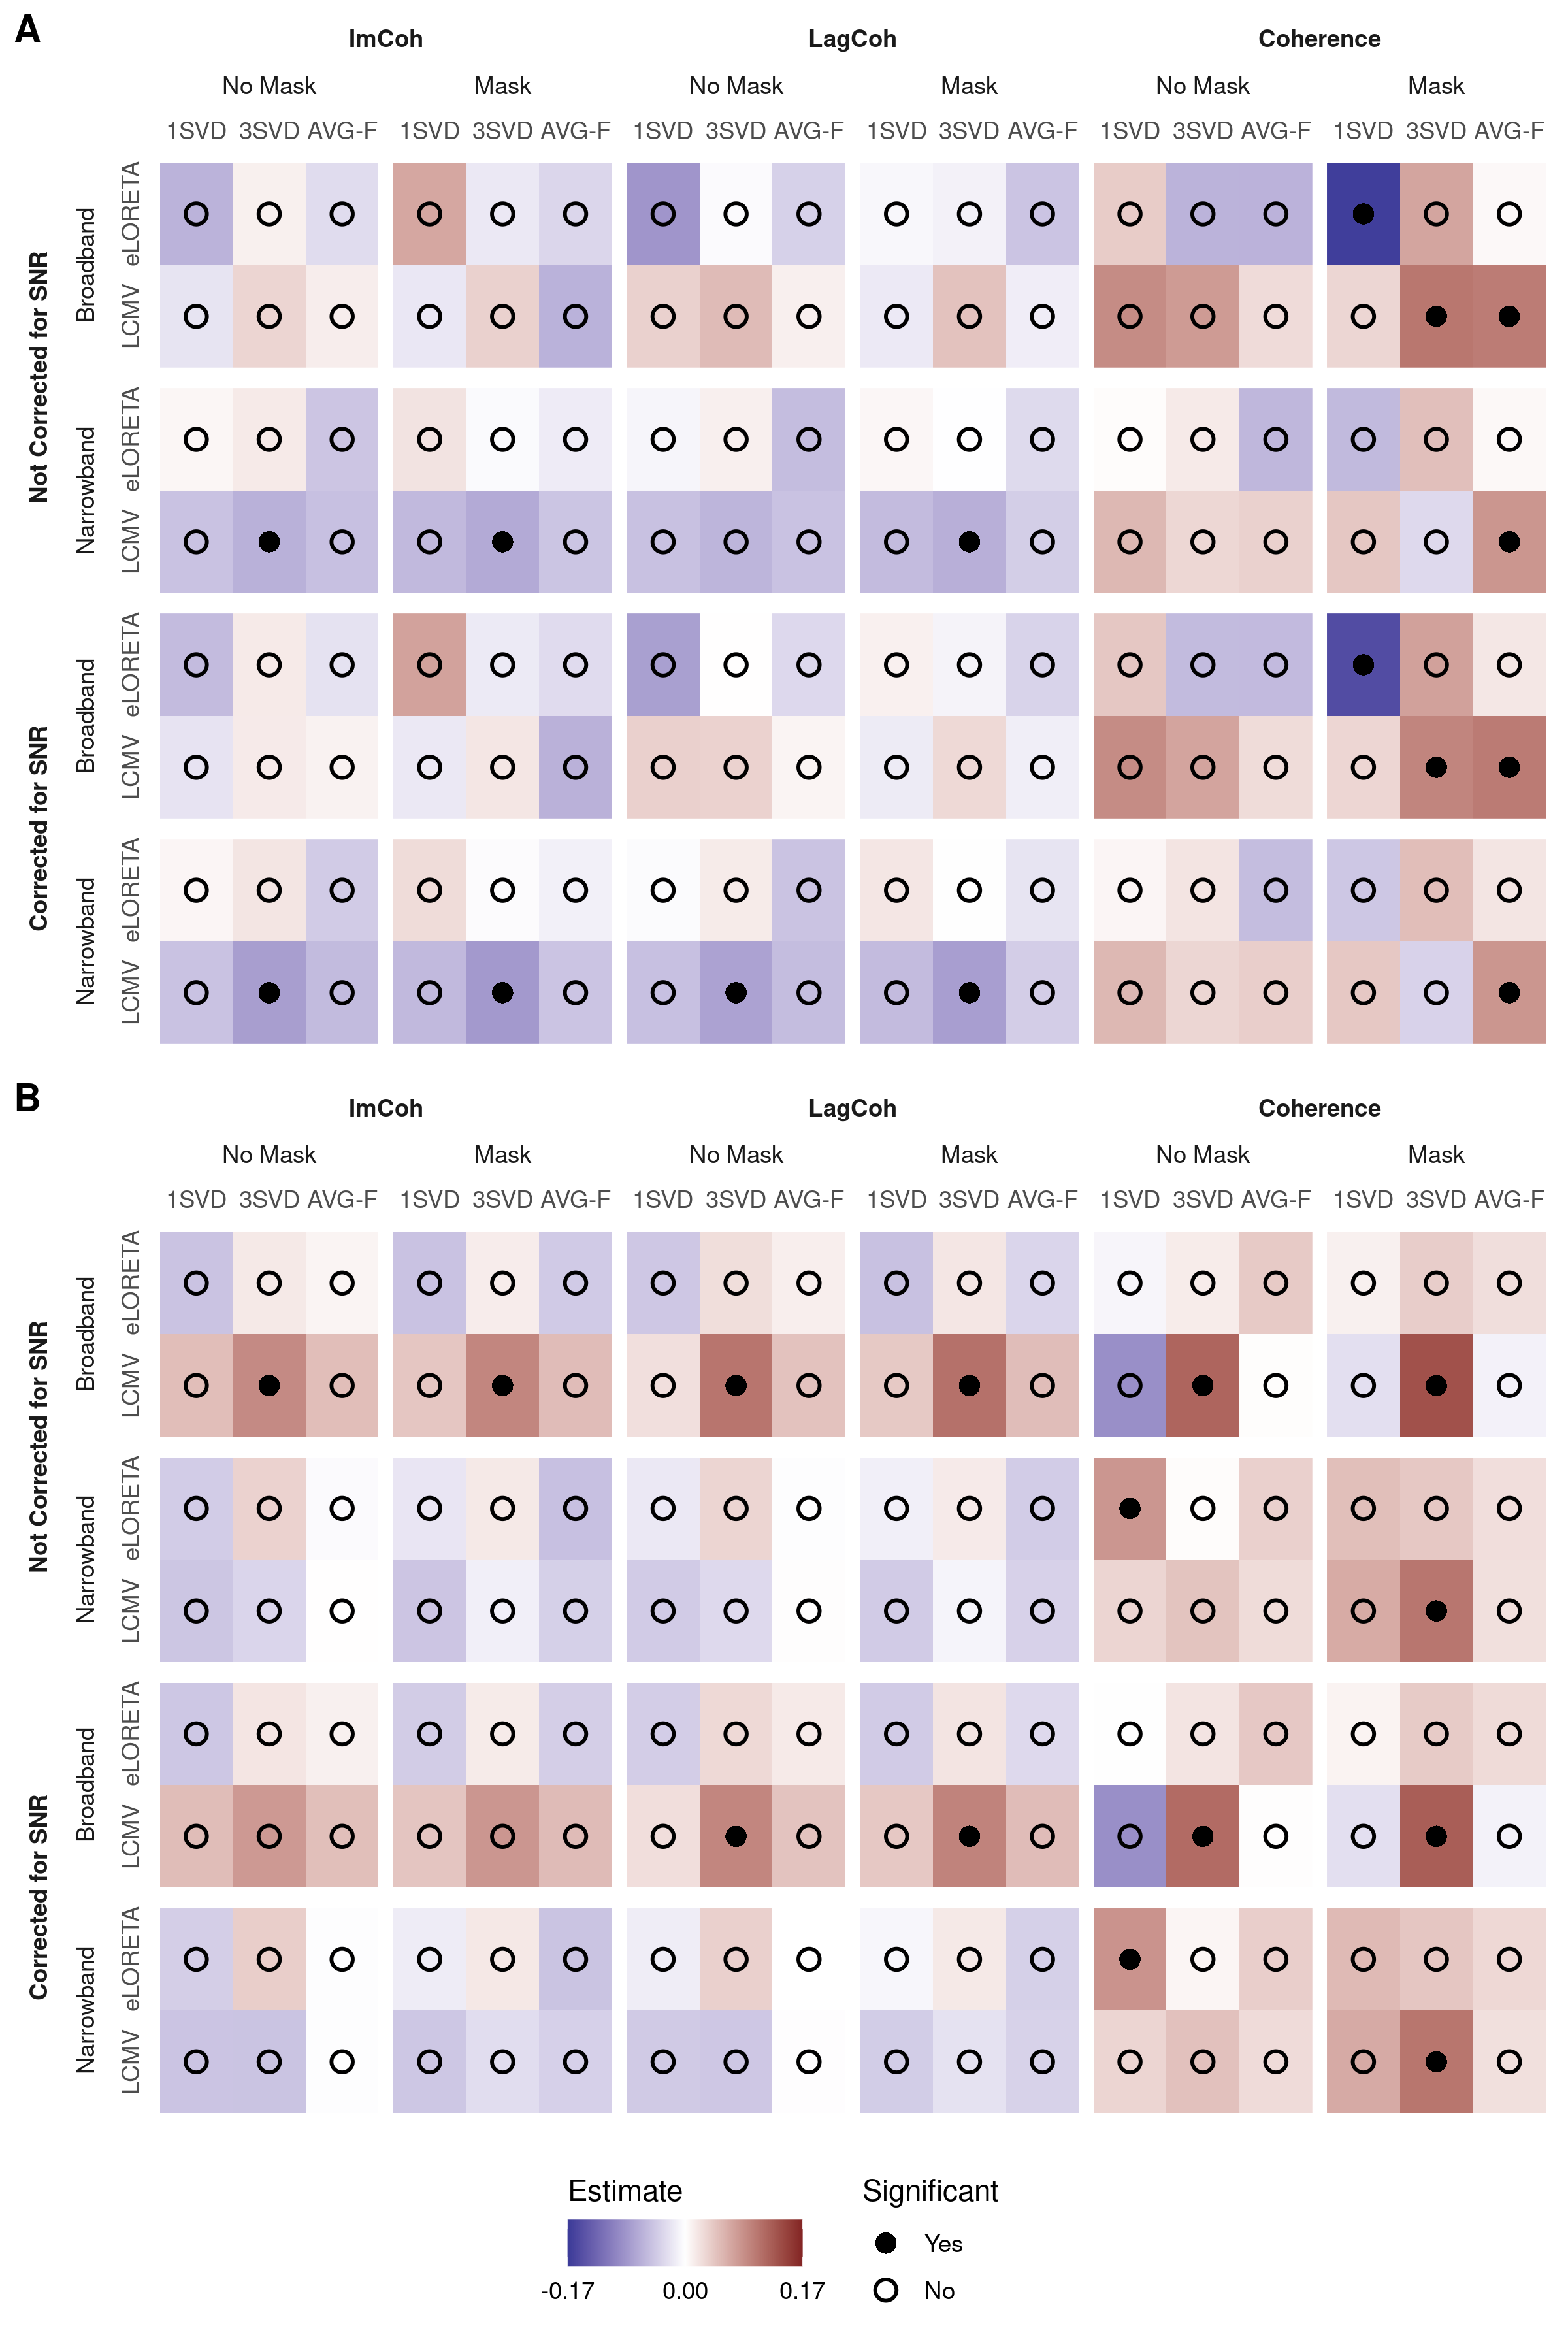
\includegraphics[width=0.9\textwidth]{fig6supp2-multiverse-connectivity-longitude.png}
    \caption{Longitudinal changes in phase synchronization throughout the BCI training. Panels (A) and (B) correspond to within- and across-hemisphere phase synchronization, respectively. Bonferroni correction for multiple ($m = \numComparisons$) comparisons was applied.}
    \label{fig:multiverse_connectivity_longitude}
\end{figure}

\begin{figure}[htbp]
    \centering
    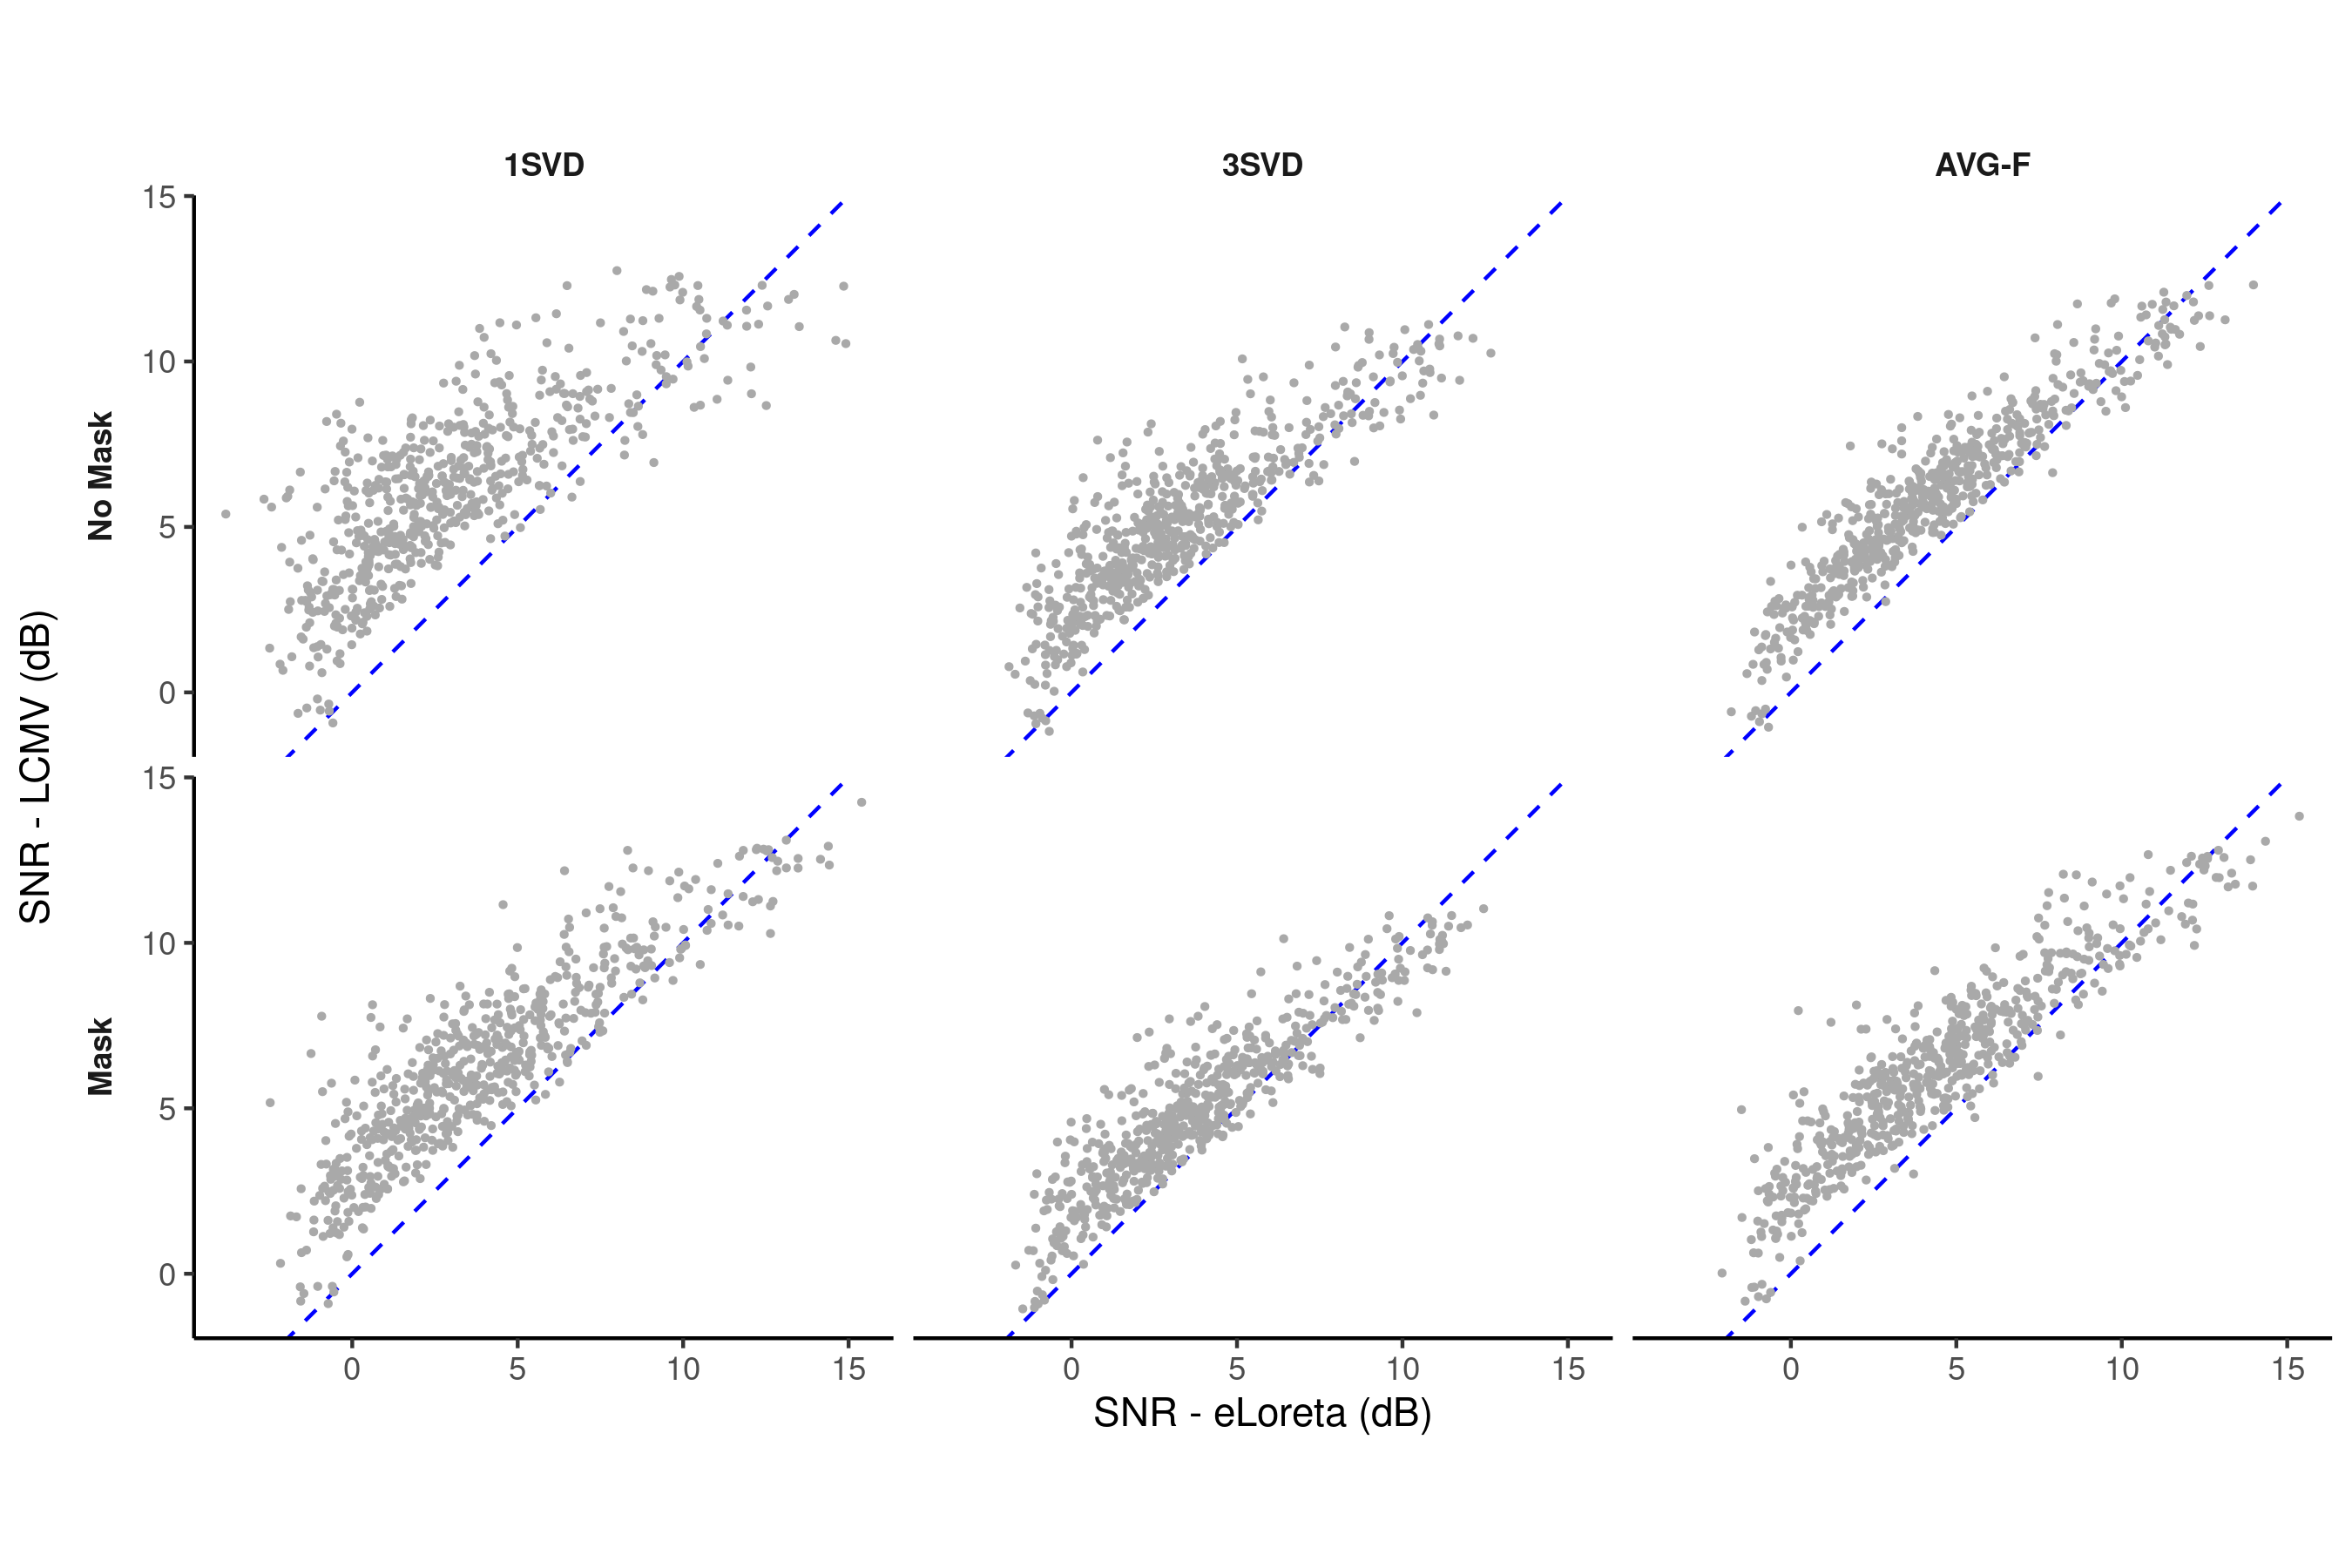
\includegraphics[width=\textwidth]{fig8supp-snr-lcmv-eloreta.png}
    \caption{The difference in SNR between pipelines that include LCMV and eLORETA was more pronounced for low values of SNR. Blue dashed lines depict the area, where values of SNR estimated with LCMV and eLORETA are equal. For points above this line, SNR is higher when LCMV is used for inverse modeling, and vice versa.}
    \label{fig:snr_lcmv_eloreta}
\end{figure}